\chapter{Fractions, Decimals, and Percentages - Parts of a Whole}

\section{Introduction: Why Learn About Fractions, Decimals, and Percentages?}
In the previous chapters, you learned about whole numbers and how to add, subtract, multiply, and divide them. But not everything in life comes in whole numbers. Sometimes, we need to talk about parts of things. This is where fractions, decimals, and percentages come in. Whether you’re measuring ingredients in a recipe, calculating a sale discount, or sharing a pizza with friends, you’re dealing with parts of a whole. These concepts are essential in daily life and will help you tackle more complex math problems down the road.

\section{What Is a Fraction?}
A fraction is a way to represent parts of a whole. It’s made up of two parts: the numerator (the top number), which tells you how many parts you have, and the denominator (the bottom number), which tells you how many equal parts the whole is divided into. For example:
\begin{itemize}
    \item In the fraction $\frac{1}{2}$, the numerator is 1, and the denominator is 2. This means we have 1 part out of 2 equal parts, or "one-half."
    \item In the fraction $\frac{3}{4}$, the numerator is 3, and the denominator is 4. This means we have 3 parts out of 4 equal parts, or "three-quarters."
\end{itemize}

\subsection{Visualizing Fractions}
You can picture fractions by thinking of a pie or pizza. Imagine cutting a pizza into 4 equal slices. Each slice is $\frac{1}{4}$ of the pizza. If you eat 2 slices, you’ve eaten 2 out of 4 parts, or $\frac{2}{4}$ of the pizza (which simplifies to $\frac{1}{2}$).

\begin{center}
    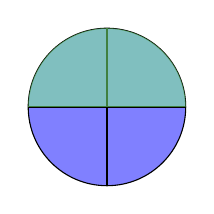
\begin{tikzpicture}
        % Draw the pizza
        \filldraw[fill=blue!50] (0,0) circle (1);
        % Draw the slices
        \draw (0,0) -- (0:0);
        \draw (0,0) -- (90:1);
        \draw (0,0) -- (180:1);
        \draw (0,0) -- (270:1);
        \draw (0,0) -- (360:1);
        % Shade the eaten slices
        \fill[green!50, opacity=0.5] (0,0) -- (0:1) arc (0:180:1) -- cycle;
    \end{tikzpicture}
    \end{center}

\subsection{Key Vocabulary}
\begin{itemize}
    \item \textbf{Proper fraction:} The numerator is smaller than the denominator (e.g., $\frac{3}{4}$).
    \item \textbf{Improper fraction:} The numerator is greater than or equal to the denominator (e.g., $\frac{5}{4}$).
    \item \textbf{Mixed number:} A whole number combined with a fraction (e.g., $1 \frac{1}{2}$).
\end{itemize}

\section{What Is a Decimal?}
A decimal is another way to represent parts of a whole, especially when working with the base-10 number system. Decimals are often used in money, measurements, and scientific data.

\subsection{Understanding Place Value in Decimals}
Just as whole numbers have place values (ones, tens, hundreds, etc.), decimals have place values for parts smaller than one:
\begin{itemize}
    \item 0.1 is one-tenth.
    \item 0.01 is one-hundredth.
    \item 0.001 is one-thousandth.
\end{itemize}

For example:
\begin{itemize}
    \item 0.5 means 5 tenths (or $\frac{1}{2}$), so it’s half of 1.
    \item 0.75 means 75 hundredths (or $\frac{3}{4}$), so it’s three-quarters of 1.
\end{itemize}

\subsection{Converting Fractions to Decimals}
We can convert fractions to decimals by dividing the numerator by the denominator. For example:
\begin{itemize}
    \item $\frac{1}{2} = 1 \div 2 = 0.5$
    \item $\frac{3}{4} = 3 \div 4 = 0.75$
\end{itemize}

\section{What Is a Percentage?}
A percentage is a way to describe parts of a whole using 100 as the reference point. It’s essentially a fraction out of 100. Percentages are extremely useful in everyday life, especially for things like discounts, taxes, and grades.

\subsection{Understanding Percentages}
\begin{itemize}
    \item 50\% means 50 out of 100, or half.
    \item 25\% means 25 out of 100, or one-quarter.
    \item 100\% means the whole thing.
\end{itemize}

\subsection{Converting Percentages to Fractions and Decimals}
\begin{itemize}
    \item 50\% = $\frac{50}{100}$ = $\frac{1}{2}$ = 0.5
    \item 25\% = $\frac{25}{100}$ = $\frac{1}{4}$ = 0.25
    \item 75\% = $\frac{75}{100}$ = $\frac{3}{4}$ = 0.75
\end{itemize}

You can also convert fractions and decimals into percentages:

\textbf{Note:}
To convert a decimal to a percentage one of two ways.
You can move the decimal point two places to the right and add a percent sign \% as shown below.

\textbf{For example:}
\begin{itemize}
    \item 0.75 becomes 75\%
    \item 0.05 becomes 5\%
    \item 1.2 becomes 120\%
\end{itemize}

To convert a decimal to a percentage, multiply by 100. For example:
\begin{enumerate}
    \item $0.2 \times 100$ = 20\%
    \item $0.65 \times 100$ = 65\%
\end{enumerate}

\section{How to Work with Fractions}
\subsection{Adding and Subtracting Fractions}
When adding or subtracting fractions, they must have the same denominator (the bottom number). Example:
\begin{itemize}
    \item $\frac{1}{3} + \frac{2}{3} = ?$ The denominators are the same, so we add the numerators: 1 + 2 = 3. The answer is $\frac{3}{3}$, which simplifies to 1.
    \item $\frac{3}{4} - \frac{1}{2} = ?$ First, find a common denominator. For $\frac{3}{4}$ and $\frac{1}{2}$, the least common denominator is 4. Convert $\frac{1}{2}$ to $\frac{2}{4}$, so now you have: $\frac{3}{4} - \frac{2}{4} = \frac{1}{4}$.
\end{itemize}

\subsection{Multiplying and Dividing Fractions}
When multiplying fractions, simply multiply the numerators and then the denominators. Example:
\begin{itemize}
    \item $\frac{1}{2} \times \frac{2}{3} = ?$ Multiply the numerators: $1 \times 2 = 2$. Multiply the denominators: $2 \times 3 = 6$. The answer is $\frac{2}{6}$, which simplifies to $\frac{1}{3}$.
\end{itemize}

When dividing fractions, multiply by the reciprocal of the second fraction (flip the numerator and denominator). Example:
\begin{itemize}
    \item $\frac{1}{2} \div \frac{2}{3} = ?$ Flip the second fraction to get $\frac{3}{2}$, and then multiply: $\frac{1}{2} \times \frac{3}{2} = \frac{3}{4}$.
\end{itemize}

\section{How to Work with Decimals}
\subsection{Adding and Subtracting Decimals}
To add or subtract decimals, make sure the decimal points are lined up. Example:
\begin{itemize}
    \item $3.25 + 1.1 = ?$ Line up the decimal points: $3.25 + 1.10 = 4.35$.
\end{itemize}

\subsection{Multiplying Decimals}
Multiply as if there were no decimal points, then count the total number of decimal places in the factors to place the decimal in the product. Example:
\begin{itemize}
    \item $0.25 \times 0.5 = ?$ Multiply $25 \times 5 = 125$. Count the decimal places: 2 in 0.25 and 1 in 0.5 (so 3 decimal places total). The answer is 0.125.
    \item $1.2 \times 2 = ?$ Multiply $12 \times 2 = 24$. There is 1 decimal place in 1.2, so the answer is 2.4.
\end{itemize}

\subsection{Dividing Decimals}
Move the decimal point in the divisor (the number you're dividing by) to make it a whole number, and move the decimal point in the dividend (the number you're dividing) the same number of places. Example:
\begin{itemize}
    \item $0.6 \div 0.2 = ?$ Move the decimal in 0.2 one place to the right (to make it 2). Move the decimal in 0.6 one place to the right (to make it 6). Now divide: $6 \div 2 = 3$.
    \item $0.75 \div 0.25 = ?$ Move the decimal in 0.25 two places to the right (to make it 25). Move the decimal in 0.75 two places to the right (to make it 75). Now divide: $75 \div 25 = 3$.
\end{itemize}

\section{How to Work with Percentages}
\subsection{Finding a Percentage of a Number}
To find a percentage of a number, multiply the number by the percentage as a decimal. Example:
\begin{itemize}
    \item $20\% of 50 = ?$ Convert 20\% to a decimal (0.20), then multiply: $50 \times 0.20 = 10$.
\end{itemize}

\subsection{Converting a Number to a Percentage}
To convert a number to a percentage, multiply it by 100 and add the \% symbol. Example:
\begin{itemize}
    \item $0.75 = ?$ Multiply: $0.75 \times 100 = 75\%$. So, 0.75 is 75\%.
\end{itemize}

\section{Practice Makes Perfect: Let’s Try Some Exercises!}
\begin{multicols}{2}
    \textbf{Fractions}
    \begin{enumerate}[label=(\alph*)]
        \item $\frac{2}{3} + \frac{1}{3} = \underline{\hspace{0.5cm}}$
        \item $\frac{3}{4} - \frac{1}{4} = \underline{\hspace{0.5cm}}$
        \item $\frac{1}{2} \times \frac{2}{3} = \underline{\hspace{0.5cm}}$
        \item $\frac{1}{2} \div \frac{2}{3} = \underline{\hspace{0.5cm}}$
        \item $\frac{3}{5} + \frac{1}{5} = \underline{\hspace{0.5cm}}$
        \item $\frac{3}{4} \div \frac{1}{2} = \underline{\hspace{0.5cm}}$
        \item $\frac{1}{3} \times \frac{3}{4} = \underline{\hspace{0.5cm}}$
        \item $\frac{1}{2} \div \frac{3}{4} = \underline{\hspace{0.5cm}}$
    \end{enumerate}
    \textbf{Decimals}
    \begin{enumerate}[label=(\alph*)]
        \item $1.2 + 0.8 = \underline{\hspace{0.5cm}}$
        \item $5.5 \div 2.5 = \underline{\hspace{0.5cm}}$
        \item $0.25 \times 0.4 = \underline{\hspace{0.5cm}}$
        \item $0.6 \div 0.2 = \underline{\hspace{0.5cm}}$
        \item $0.75 + 0.25 = \underline{\hspace{0.5cm}}$
        \item $1.5 \div 0.5 = \underline{\hspace{0.5cm}}$
        \item $0.75 \times 0.25 = \underline{\hspace{0.5cm}}$
        \item $1.2 \div 0.4 = \underline{\hspace{0.5cm}}$
    \end{enumerate}
\end{multicols}
\begin{center}
    \textbf{Percentages}
    \begin{enumerate}[label=(\alph*)]
        \item 25\% of 80 = $\underline{\hspace{0.5cm}}$
        \item Convert 0.6 to a percentage = $\underline{\hspace{0.5cm}}$
        \item Convert $\frac{1}{5}$ to a percentage = $\underline{\hspace{0.5cm}}$
        \item Convert 50\% to a fraction = $\underline{\hspace{0.5cm}}$
        \item 20\% of 60 = $\underline{\hspace{0.5cm}}$
        \item Convert 0.75 to a percentage = $\underline{\hspace{0.5cm}}$
        \item Convert $\frac{3}{4}$ to a percentage = $\underline{\hspace{0.5cm}}$
        \item 75\% of 40 = $\underline{\hspace{0.5cm}}$
    \end{enumerate}
\end{center}

\section{Real-Life Applications of Fractions, Decimals, and Percentages}
\subsection{Cooking}
Recipes often use fractions (e.g., $\frac{1}{2}$ cup of sugar). If you’re doubling the recipe, you need to multiply those fractions.

\subsection{Shopping}
You see a 30\% discount on an item. To find the sale price, you need to calculate 30\% of the original price.

\subsection{Money}
If you earn \$50 and save 20\%, how much money are you saving? Find 20\% of \$50 to see that you’re saving \$10.

\section{Converting Between Fractions, Decimals, and Percentages}
Understanding how to convert between fractions, decimals, and percentages is essential. These forms all represent parts of a whole, but they are useful in different situations. Let's explore how to move between these forms.

\subsection{Converting Fractions to Decimals}
To convert a fraction to a decimal, divide the numerator (top number) by the denominator (bottom number). Example:
\begin{itemize}
    \item Convert $\frac{3}{4}$ to a decimal: $\frac{3}{4} = 3 \div 4 = 0.75$
    \item Convert $\frac{1}{2}$ to a decimal: $\frac{1}{2} = 1 \div 2 = 0.5$
\end{itemize}

\subsection{Converting Decimals to Fractions}
To convert a decimal to a fraction, write the decimal as the numerator and use the place value of the decimal as the denominator. Example:
\begin{itemize}
    \item Convert 0.25 to a fraction: $0.25 = \frac{25}{100}$, which simplifies to $\frac{1}{4}$
    \item Convert 0.6 to a fraction: $0.6 = \frac{6}{10}$, which simplifies to $\frac{3}{5}$
\end{itemize}

\subsection{Converting Fractions to Percentages}
To convert a fraction to a percentage, first divide the numerator by the denominator to get a decimal. Then, multiply the decimal by 100 to find the percentage. Example:
\begin{itemize}
    \item Convert $\frac{3}{5}$ to a percentage: $\frac{3}{5} = 3 \div 5 = 0.6$ $0.6 \times 100 = 60\%$
    \item Convert $\frac{7}{8}$ to a percentage: $\frac{7}{8} = 7 \div 8 = 0.875$ $0.875 \times 100 = 87.5\%$
\end{itemize}

\subsection{Converting Percentages to Fractions}
To convert a percentage to a fraction, write the percentage as the numerator and 100 as the denominator, then simplify if possible. Example:
\begin{itemize}
    \item Convert 75\% to a fraction: $75\% = \frac{75}{100}$, which simplifies to $\frac{3}{4}$
    \item Convert 20\% to a fraction: $20\% = \frac{20}{100}$, which simplifies to $\frac{1}{5}$
\end{itemize}

\subsection{Converting Decimals to Percentages}
To convert a decimal to a percentage, multiply the decimal by 100 and add the \% sign. Example:
\begin{itemize}
    \item Convert 0.85 to a percentage: $0.85 \times 100 = 85\%$
    \item Convert 0.125 to a percentage: $0.125 \times 100 = 12.5\%$
\end{itemize}

\subsection{Converting Percentages to Decimals}
To convert a percentage to a decimal, divide by 100 or move the decimal point two places to the left. Example:
\begin{itemize}
    \item Convert 50\% to a decimal: $50 \div 100 = 0.50$
    \item Convert 12.5\% to a decimal: $12.5 \div 100 = 0.125$
\end{itemize}

\section{Chapter Summary}
Fractions represent parts of a whole, and you can add, subtract, multiply, and divide them just like whole numbers.
Decimals are another way to express parts of a whole, especially when working in the base-10 system. You can perform arithmetic operations with decimals just as you do with whole numbers.
Percentages represent parts of a whole in terms of 100 and are useful in many real-life applications such as discounts, grades, and statistics.
Converting between fractions, decimals, and percentages is an essential skill for understanding and comparing parts of a whole in different forms.

\subsection{Challenge Question:}
\begin{enumerate}[label=(\alph*)]
    \item You bought a sweater for \$48 after a 20\% discount. What was the original price of the sweater? (Hint: If you received a 20\% discount, you paid 80\% of the original price.)
    \begin{itemize}
        \item 20\% of the original price = \$48 (the discount)
        \item 80\% of the original price = \$48 (what you paid)
        \item Let x = the original price
        \item $0.80x = \$48$
        \item $x = \$48 \div 0.80 = \$60$
        \item The original price of the sweater was \$60.
        \item Check: 20\% of \$60 = \$12 (the discount), so \$60 - \$12 = \$48 (the sale price).
        \item The original price of the sweater was \$60.
    \end{itemize}
    \item You have a piece of ribbon that is 2.5 meters long. You need to cut it into pieces that are each 0.4 meters long. How many pieces of ribbon can you cut, and how much ribbon will be left over?
        \begin{itemize}
            \item Total length of ribbon = 2.5 meters
            \item Length of each piece = 0.4 meters
            \item Number of pieces = $2.5 \div 0.4 = 6.25$
            \item You can cut 6 full pieces of ribbon.
            \item Leftover ribbon = $2.5 - (6 \times 0.4) = 2.5 - 2.4 = 0.1$ meters
            \item You will have 0.1 meters of ribbon left over.
        \end{itemize}
    \item You scored 18 out of 20 on a test. What percentage did you score?
        \begin{itemize}
            \item Score = 18 out of 20
            \item Percentage = $\frac{18}{20} \times 100 = 90\%$
            \item You scored 90\% on the test.
        \end{itemize}
    \item You have a recipe that calls for $\frac{3}{4}$ cup of sugar. If you want to make a double batch, how much sugar will you need?
        \begin{itemize}
            \item Original recipe = $\frac{3}{4}$ cup of sugar
            \item Double batch = $2 \times \frac{3}{4} = \frac{6}{4} = 1 \frac{1}{2}$ cups of sugar
            \item You will need 1 $\frac{1}{2}$ cups of sugar for a double batch.
        \end{itemize}
    \item You have a pizza that is divided into 8 slices. If you eat 3 slices, what percentage of the pizza have you eaten?
        \begin{itemize}
            \item Slices eaten = 3 out of 8
            \item Percentage eaten = $\frac{3}{8} \times 100 = 37.5\%$
            \item You have eaten 37.5\% of the pizza.
            \item Check: 3 slices out of 8 is the same as $\frac{3}{8}$, which is 37.5\%.
            \item You have eaten 37.5\% of the pizza.
        \end{itemize}
    \item You have a jar of marbles with 30 red marbles and 20 blue marbles. What percentage of the marbles are red?
        \begin{itemize}
            \item Total marbles = 30 red + 20 blue = 50 marbles
            \item Percentage of red marbles = $\frac{30}{50} \times 100 = 60\%$
            \item 60\% of the marbles are red.
        \end{itemize}
\end{enumerate}